% Provenance (never printed): cycle 4 SVT/physique, "La planete Terre,
% l'environnement": uneven heating of the Earth, movements of the
% atmosphere, the global circulation and the climate zones; see
% sources/book1/PROVENANCE.md. Book 1, grade 8, chapter 2.
% Vocabulary guard: owns convection cell (atmospheric, descriptive), sea
% breeze and land breeze, the global winds, the global circulation. The
% Coriolis effect is told as "the Earth's rotation deflects"; Hadley and
% Ferrel cells and the intertropical convergence zone are named in prose
% only (Book 3 owns them); mantle convection is Book 2's.
\chapter{Os ventos e a circulação geral}\label{ch:g8:winds-global-circulation}

Durante séculos, os veleiros que saíam dos portos da Europa e da África
para as Américas contavam com um vento constante vindo do leste, que sopra
dos dois lados do \omterm{def:g3:continents-and-oceans:equator}{equador} e os levava através do Atlântico. Os marinheiros
do mundo inteiro o conheciam, e o comércio inicial com as Américas
dependia dele: é o \emph{alísio}. Ainda hoje, os navios de carga usam os
\omterm{def:g8:winds-global-circulation:global-winds}{alísios}, e as correntes oceânicas que eles movem, para encurtar as suas
viagens.
% ledger: nos:trade-winds

\begin{omfigure}
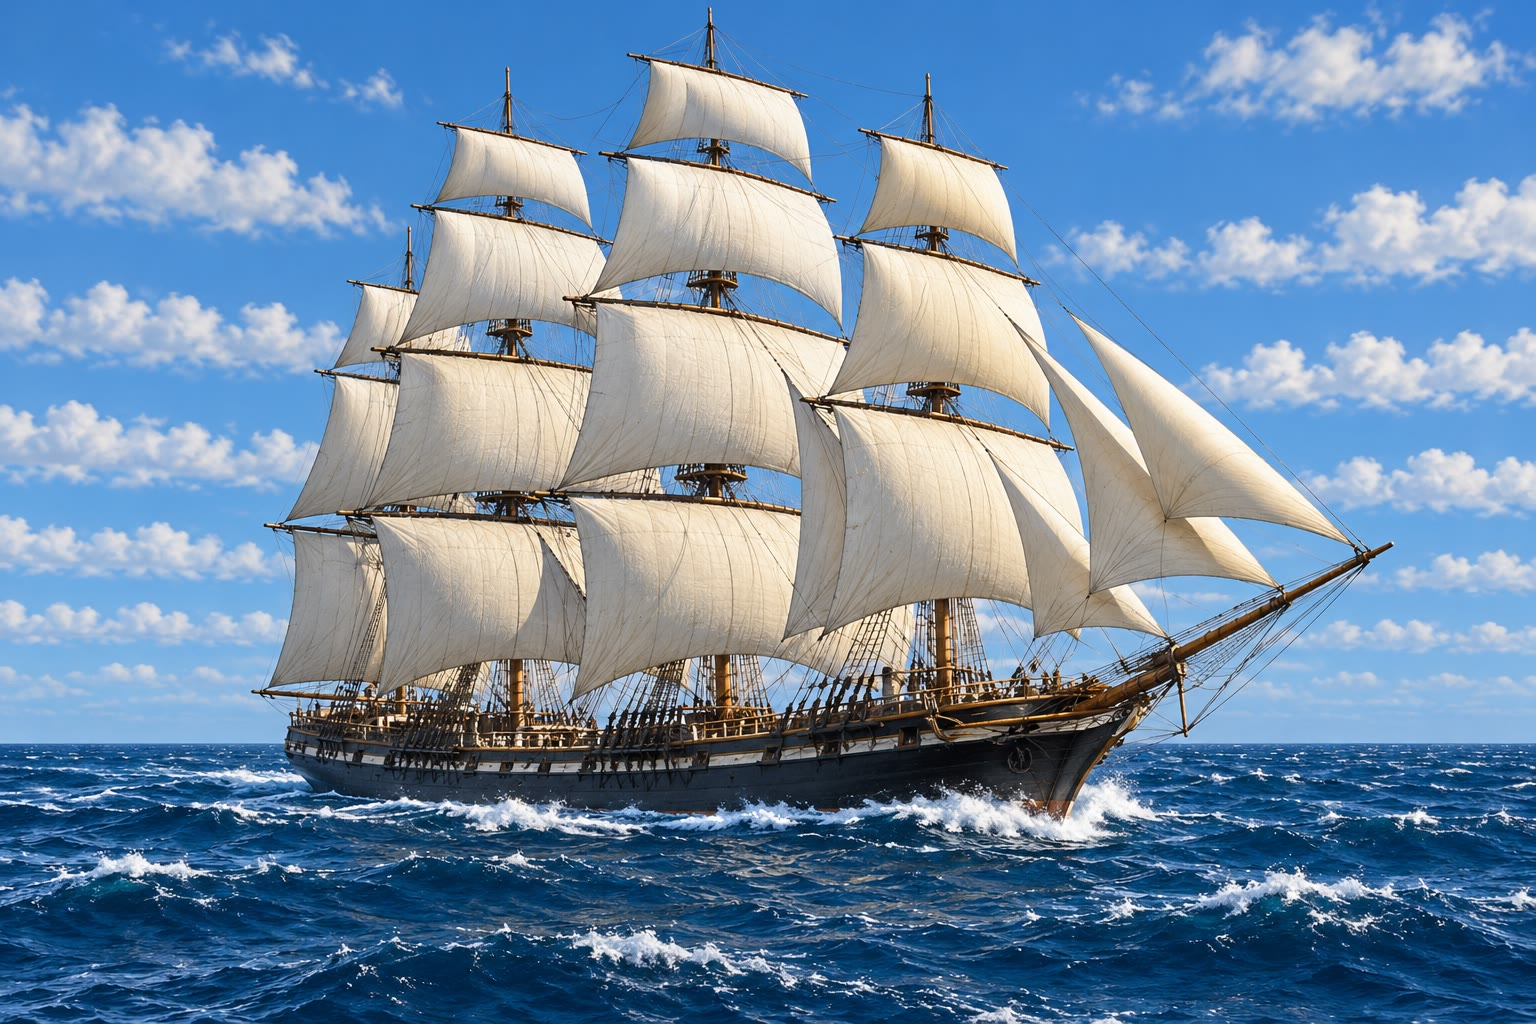
\includegraphics[width=0.62\linewidth]{images/book1/ai/g8-sailing-ship.jpg}

{\small Um veleiro navegando com um vento constante pela popa, em pleno
\omterm{def:g2:water-on-earth:ocean}{oceano} (ilustração de uma cena genérica feita por IA).}
\label{fig:g8:winds-global-circulation:ship}
\end{omfigure}

Por que o alísio sopra do leste, e sempre nos mesmos lugares? Por que há
\omterm{def:g5:weather-and-climate:desert}{desertos} perto dos \omterm{def:g5:weather-and-climate:tropics}{trópicos} e florestas tropicais úmidas perto do \omterm{def:g3:continents-and-oceans:equator}{equador}?
A resposta começa no Sol.

\begin{recall}
O vento é ar em movimento (os livros de física). O ar faz pressão sobre
tudo o que ele toca, e a pressão cai com a \omterm{def:g4:world-physical-map:altitude}{altitude}
(\cref{ch:g8:the-atmosphere}). O \omterm{def:g1:watching-the-weather:weather}{tempo} meteorológico acontece na
\omterm{def:g8:the-atmosphere:layers}{troposfera}, a camada mais baixa da atmosfera. A Terra tem \omterm{def:g5:weather-and-climate:climate-zone}{zonas
climáticas}: quente e úmida perto do \omterm{def:g3:continents-and-oceans:equator}{equador}, com florestas tropicais
úmidas; \omterm{def:g5:weather-and-climate:desert}{desertos} quentes e áridos perto dos \omterm{def:g5:weather-and-climate:tropics}{trópicos}; zonas temperadas, e
depois frias, em direção aos \omterm{def:g3:continents-and-oceans:poles}{polos} (\cref{ch:g5:weather-and-climate}).
\end{recall}

\section{O Sol aquece a Terra de maneira desigual}

Ao meio-dia de um dia de equinócio, o Sol fica bem a pino no \omterm{def:g3:continents-and-oceans:equator}{equador}. Os
seus raios chegam ali quase na vertical e caem numa pequena área do chão.
Mais ao norte ou mais ao sul, os mesmos raios chegam inclinados e se
espalham por uma área maior: cada metro quadrado recebe menos da sua
energia. Na \omterm{def:g6:latitude-longitude:latitude}{latitude} \ang{60}, o mesmo feixe cobre o dobro do chão que
cobre no \omterm{def:g3:continents-and-oceans:equator}{equador}, então cada metro quadrado recebe a metade.
% ledger: (geometry: figdata/grade-8/sunlight_spread.py, spread = 1/cos(latitude))

\begin{omfigure}
\begin{tikzpicture}[font=\footnotesize]
  \def\R{2.6}\def\w{0.2}
  \fill[blue!10] (0,0) circle (\R);
  \draw (0,0) circle (\R);
  \draw[black!50] (-\R,0) -- (\R,0);
  \draw[black!40, dashed] (0,0) -- (60:\R);
  \draw[black!40] (0,0) ++(0:0.7) arc (0:60:0.7);
  \node at (25:0.95) {\ang{60}};
  \node[anchor=east, black!60] at (-\R-0.05,0) {equador};
  % beam at the equator: rays between y = -w and y = w
  \foreach \y in {-0.2,-0.1,0,0.1,0.2} {
    \pgfmathsetmacro{\x}{sqrt(\R*\R-\y*\y)}
    \draw[orange!80!black, -{Stealth[length=1.6mm]}] (6.2,\y) -- (\x+0.03,\y);}
  \draw[omThm, line width=2.2pt] ({sqrt(\R*\R-0.35*0.35)},-0.35) arc ({asin(-\w/\R)}:{asin(\w/\R)}:\R);
  % beam near 60 degrees: rays between y = R sin 60 - w and + w
  \pgfmathsetmacro{\yc}{\R*sin(60)}
  \foreach \d in {-0.2,-0.1,0,0.1,0.2} {
    \pgfmathsetmacro{\y}{\yc+\d}
    \pgfmathsetmacro{\x}{sqrt(\R*\R-\y*\y)}
    \draw[orange!80!black, -{Stealth[length=1.6mm]}] (6.2,\y) -- (\x+0.03,\y);}
  \draw[omThm, line width=2.2pt] ({sqrt(\R*\R-(\yc-\w)^2)},\yc-\w) arc ({asin((\yc-\w)/\R)}:{asin((\yc+\w)/\R)}:\R);
  \node[anchor=west, align=left] at (6.3,0) {o mesmo feixe\\numa pequena área};
  \node[anchor=west, align=left] at (6.3,\yc) {o mesmo feixe espalhado\\pelo dobro do chão};
\end{tikzpicture}

{\small Dois feixes iguais de luz do Sol ao meio-dia de um equinócio. No
\omterm{def:g3:continents-and-oceans:equator}{equador}, eles caem bem na vertical numa pequena área (traço grosso); a
\ang{60} de \omterm{def:g6:latitude-longitude:latitude}{latitude}, eles chegam inclinados e cobrem o dobro do chão.}
% ledger: (geometry: figdata/grade-8/sunlight_spread.py)
\label{fig:g8:winds-global-circulation:beams}
\end{omfigure}

\begin{center}\small
\begin{tabular}{|l|c|c|c|c|c|}
\hline
\omterm{def:g6:latitude-longitude:latitude}{latitude} & \ang{0} & \ang{30} & \ang{45} & \ang{60} & \ang{75} \\
\hline
chão coberto pelo mesmo feixe & 1 & 1.15 & 1.41 & 2 & 3.86 \\
\hline
energia por metro quadrado (\% da do \omterm{def:g3:continents-and-oceans:equator}{equador}) & 100 & 87 & 71 & 50 & 26 \\
\hline
\end{tabular}
\end{center}
% ledger: (figdata/grade-8/sunlight_spread.py main table)

Enquanto a Terra gira em volta do Sol, o seu eixo inclinado faz o Sol a
pino se deslocar entre os dois \omterm{def:g5:weather-and-climate:tropics}{trópicos}, o que dá as estações (os livros
de física); mas, o ano todo, as regiões perto do \omterm{def:g3:continents-and-oceans:equator}{equador} recebem muito
mais energia que as que ficam perto dos \omterm{def:g3:continents-and-oceans:poles}{polos}. Esse aquecimento desigual
é o principal motor dos ventos: a atmosfera leva o ar quente em direção
aos \omterm{def:g3:continents-and-oceans:poles}{polos} e o ar frio em direção ao \omterm{def:g3:continents-and-oceans:equator}{equador}.
% ledger: mo:global-circ

\section{O ar que sobe e o ar que desce}

O ar quente é mais leve que o ar frio: ele sobe, e o ar mais fresco em
volta vem ocupar o seu lugar. Onde o ar sobe, ele faz menos pressão sobre
o chão: a pressão ali é baixa. Onde o ar desce, ele faz mais pressão: a
pressão é alta. No chão, o vento sopra da alta pressão para a baixa
pressão. Subindo, esfriando, descendo e voltando, o ar gira num circuito.
% ledger: jetstream:sea-breeze, mo:three-cells

\begin{definition}[Célula de convecção]\label{def:g8:winds-global-circulation:convection-cell}
Uma \emph{célula de convecção}\index{celula de conveccao@célula de convecção} na atmosfera é um
circuito de ar em movimento: o ar aquecido por baixo sobe, se espalha lá
no alto, esfria e desce em outro lugar, e volta ao longo do chão até onde
ele subiu. Embaixo do ar que sobe, a pressão é baixa; embaixo do ar que
desce, ela é alta.
\end{definition}
% ledger: jetstream:sea-breeze, mo:three-cells

\begin{inthelab}[O ar quente sobe]
Dentro de casa, recorte uma espiral numa folha de papel fino, como a casca
de uma maçã, e pendure-a pelo centro num fio. Segure-a bem acima de um
aquecedor quente, no inverno (nunca acima de uma chama ou de uma vela):
ela começa a girar devagar. O ar aquecido pelo aquecedor sobe e empurra a
espiral. Segure-a perto de uma janela fria: ela gira no outro sentido, ou
não gira?
\end{inthelab}

As menores \omterm{def:g8:winds-global-circulation:convection-cell}{células de convecção} podem ser sentidas num dia de sol na
praia. A terra e o \omterm{def:g2:water-on-earth:ocean}{mar} recebem a mesma luz do Sol, mas os raios do Sol não
penetram fundo no chão, enquanto o \omterm{def:g2:water-on-earth:ocean}{mar} espalha o seu calor por uma camada
espessa de água. Então a terra esquenta muito mais de dia, e esfria muito
mais à noite.
% ledger: jetstream:sea-breeze

\begin{omfigure}
\begin{tikzpicture}[font=\footnotesize, >={Stealth[length=2mm]}]
  \foreach \px/\title/\dir in {0/{De dia: a brisa marítima}/1, 8.3/{À noite: a brisa terrestre}/-1} {
    \begin{scope}[xshift=\px cm]
      \fill[omSea] (0,0) rectangle (3.5,0.45);
      \fill[omLithAlluv] (3.5,0) -- (3.5,0.45) -- (7,0.75) -- (7,0) -- cycle;
      \draw (0,0.45) -- (3.5,0.45) -- (7,0.75);
      \node[anchor=south] at (3.5,3.25) {\textbf{\title}};
      \node at (1.75,0.22) {mar};
      \node at (5.6,0.3) {terra};
    \end{scope}}
  % day loop: surface sea -> land, rise over land, return aloft, sink over sea
  \draw[->, omDef, line width=1.1pt] (1.2,0.8) -- (5.2,0.95);
  \draw[->, omThm, line width=1.1pt] (5.8,1.1) -- (5.8,2.4);
  \draw[->, black!60, line width=1.1pt] (5.2,2.75) -- (1.2,2.75);
  \draw[->, omDef, line width=1.1pt] (0.6,2.4) -- (0.6,1.1);
  \node[omDef] at (3.2,1.25) {brisa marítima};
  \node at (0.6,0.75) {\textbf{H}};
  \node at (5.8,0.95) {\textbf{L}};
  \fill[yellow!80!orange] (6.6,2.7) circle (0.25);
  \node[anchor=north, align=center] at (1.75,-0.1) {mar mais fresco};
  \node[anchor=north, align=center] at (5.3,-0.1) {terra mais quente};
  % night loop: surface land -> sea, rise over sea, return aloft, sink over land
  \begin{scope}[xshift=8.3cm]
    \draw[->, omDef, line width=1.1pt] (5.2,1.0) -- (1.2,0.8);
    \draw[->, omThm, line width=1.1pt] (0.6,1.1) -- (0.6,2.4);
    \draw[->, black!60, line width=1.1pt] (1.2,2.75) -- (5.2,2.75);
    \draw[->, omDef, line width=1.1pt] (5.8,2.4) -- (5.8,1.15);
    \node[omDef] at (3.2,1.3) {brisa terrestre};
    \node at (0.6,0.75) {\textbf{L}};
    \node at (5.8,1.0) {\textbf{H}};
    \fill[black!25] (6.6,2.7) circle (0.25); \fill[white] (6.72,2.78) circle (0.21);
    \node[anchor=north, align=center] at (1.75,-0.1) {mar mais quente};
    \node[anchor=north, align=center] at (5.3,-0.1) {terra mais fria};
  \end{scope}
\end{tikzpicture}

{\small A \omterm{def:g8:winds-global-circulation:breezes}{brisa marítima} e a \omterm{def:g8:winds-global-circulation:breezes}{brisa terrestre}: duas pequenas \omterm{def:g8:winds-global-circulation:convection-cell}{células de
convecção} que giram em sentidos opostos. Setas vermelhas: ar quente que
sobe; H e L: alta e baixa pressão no chão. De dia, o circuito chega a
1000 a \qty{1500}{m} de altura.}
% ledger: jetstream:sea-breeze
\label{fig:g8:winds-global-circulation:breezes}
\end{omfigure}

\begin{definition}[Brisa marítima e brisa terrestre]\label{def:g8:winds-global-circulation:breezes}
Uma \emph{brisa marítima}\index{brisa maritima@brisa marítima} é um vento que sopra do \omterm{def:g2:water-on-earth:ocean}{mar} para
a terra de dia, quando a terra está mais quente que o \omterm{def:g2:water-on-earth:ocean}{mar}. Uma
\emph{brisa terrestre}\index{brisa terrestre} sopra da terra para o \omterm{def:g2:water-on-earth:ocean}{mar} à
noite, quando a terra ficou mais fria que o \omterm{def:g2:water-on-earth:ocean}{mar}.
\end{definition}
% ledger: jetstream:sea-breeze

\begin{omfigure}
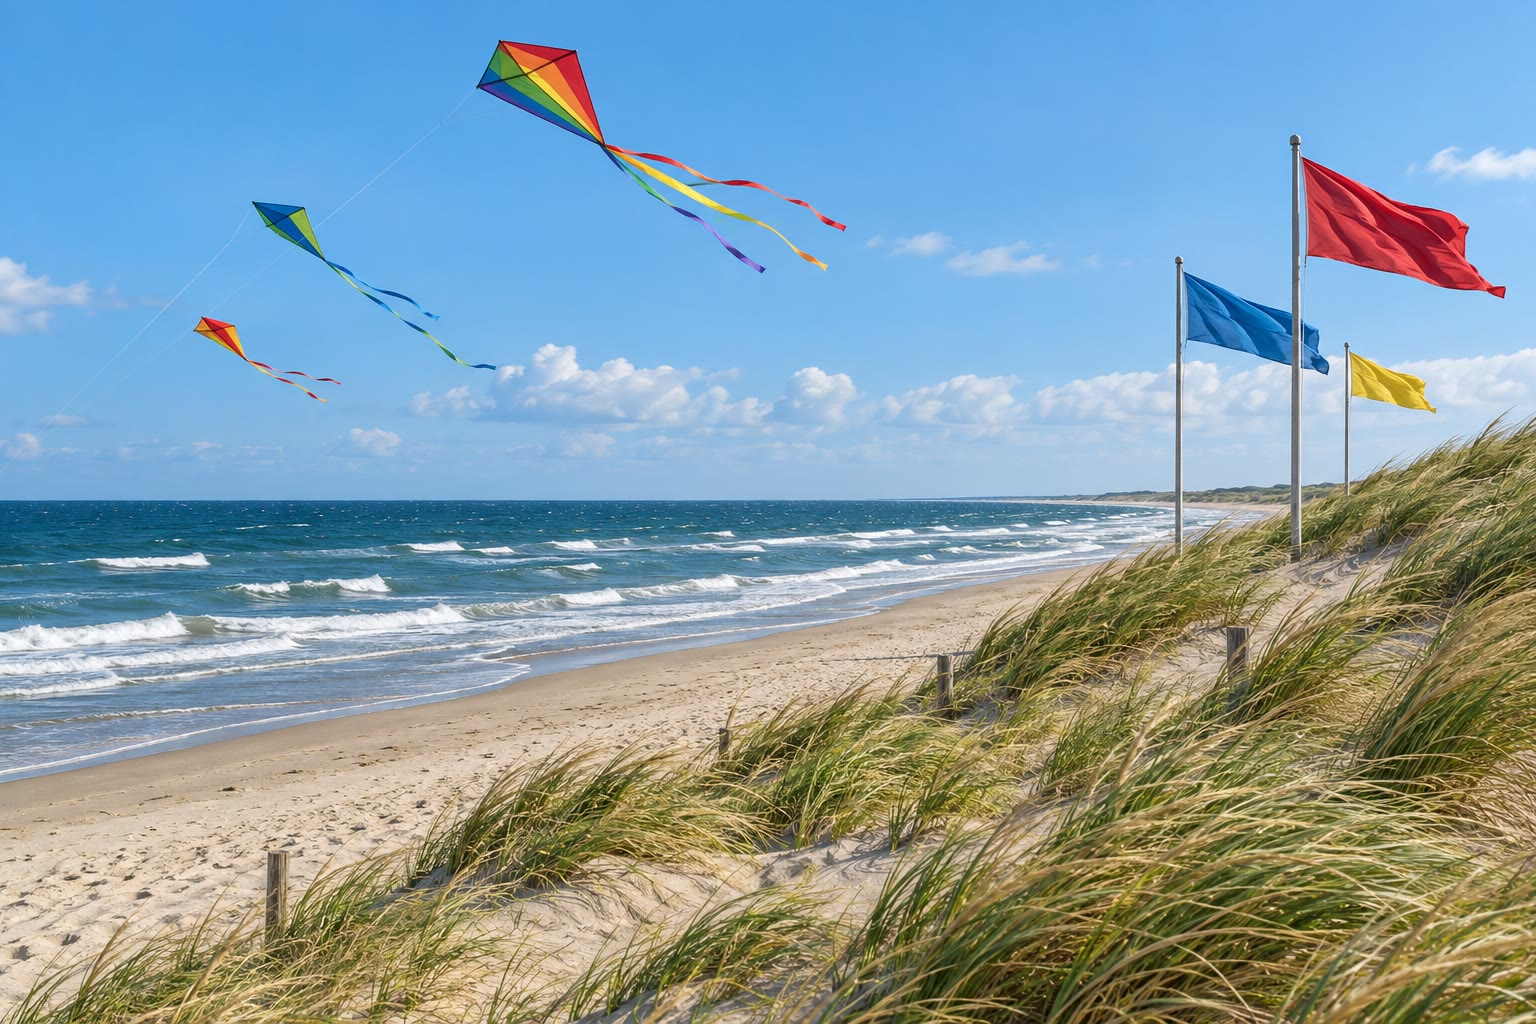
\includegraphics[width=0.55\linewidth]{images/book1/ai/g8-beach-kites.jpg}

{\small Pipas voando no vento da tarde numa praia (ilustração de uma cena
genérica feita por IA).}
\label{fig:g8:winds-global-circulation:kites}
\end{omfigure}

\section{Os ventos globais}

A mesma coisa acontece na escala da Terra inteira. Perto do \omterm{def:g3:continents-and-oceans:equator}{equador}, o ar
fortemente aquecido sobe; ele se espalha lá no alto em direção aos \omterm{def:g3:continents-and-oceans:poles}{polos}
e desce de novo perto de \ang{30} de \omterm{def:g6:latitude-longitude:latitude}{latitude}. Na média de muitos anos, a
\omterm{def:g8:the-atmosphere:layers}{troposfera} de cada \omterm{def:g3:continents-and-oceans:equator}{hemisfério} gira em três grandes \omterm{def:g8:winds-global-circulation:convection-cell}{células de convecção}:
uma do \omterm{def:g3:continents-and-oceans:equator}{equador} até cerca de \ang{30}, uma de cerca de \ang{30} até cerca
de \ang{60}, e uma de cerca de \ang{60} até o \omterm{def:g3:continents-and-oceans:poles}{polo}. Os meteorologistas as
chamam de células de Hadley, de Ferrel e polar. Os seus limites se
deslocam com as estações, e a célula do meio é uma média aproximada de
muitas \omterm{def:g5:natural-hazards:storm}{tempestades} que passam.
% ledger: mo:three-cells, mo:global-circ, nos:doldrums

Os ventos que sopram no chão iriam diretamente da alta para a baixa
pressão se a Terra não girasse. Como a Terra gira, o ar em movimento é
desviado: para a direita no \omterm{def:g3:continents-and-oceans:equator}{hemisfério norte}, para a esquerda no
\omterm{def:g3:continents-and-oceans:equator}{hemisfério sul}. Então o ar que volta para o \omterm{def:g3:continents-and-oceans:equator}{equador} não vem do norte, mas
do nordeste no \omterm{def:g3:continents-and-oceans:equator}{hemisfério norte} e do sudeste no \omterm{def:g3:continents-and-oceans:equator}{hemisfério sul}.
% ledger: mo:global-circ, nos:trade-winds

\begin{definition}[Os ventos globais]\label{def:g8:winds-global-circulation:global-winds}
Os ventos de superfície que sopram com mais frequência em cada faixa de \omterm{def:g6:latitude-longitude:latitude}{latitude} são:
\begin{itemize}
  \item os \emph{alísios}\index{alisios@alísios}, entre o \omterm{def:g3:continents-and-oceans:equator}{equador} e cerca
        de \ang{30}, que sopram do nordeste no \omterm{def:g3:continents-and-oceans:equator}{hemisfério norte} e do
        sudeste no \omterm{def:g3:continents-and-oceans:equator}{hemisfério sul};
  \item os \emph{ventos de oeste}\index{ventos de oeste}, entre cerca de
        \ang{30} e \ang{60}, que sopram do oeste (do sudoeste no
        \omterm{def:g3:continents-and-oceans:equator}{hemisfério norte}, do noroeste no \omterm{def:g3:continents-and-oceans:equator}{hemisfério sul});
  \item os \emph{ventos polares de leste}\index{ventos polares de leste}, entre cerca de
        \ang{60} e os \omterm{def:g3:continents-and-oceans:poles}{polos}, que sopram do leste.
\end{itemize}
\end{definition}
% ledger: nos:trade-winds, mo:three-cells, mo:global-circ

\begin{omfigure}
\begin{tikzpicture}[font=\scriptsize, >={Stealth[length=1.8mm]}]
  \def\R{3}
  \fill[blue!8] (0,0) circle (\R);
  \draw (0,0) circle (\R);
  \draw[black!45] (-\R,0) -- (\R,0);
  \foreach \l in {-60,-30,30,60} {
    \pgfmathsetmacro{\y}{\R*sin(\l)}
    \pgfmathsetmacro{\x}{\R*cos(\l)}
    \draw[black!45, dashed] (-\x,\y) -- (\x,\y);}
  % surface winds: NE trades, SW westerlies, NE polar easterlies (north); mirrored south
  \foreach \x in {-1.8,-0.6,0.6,1.8} {
    \draw[->, omThm, line width=0.9pt] (\x+0.35,0.95) -- (\x-0.35,0.55);
    \draw[->, omThm, line width=0.9pt] (\x+0.35,-0.95) -- (\x-0.35,-0.55);}
  \foreach \x in {-1.2,0,1.2} {
    \draw[->, omDef, line width=0.9pt] (\x-0.35,1.7) -- (\x+0.35,2.02);
    \draw[->, omDef, line width=0.9pt] (\x-0.35,-1.7) -- (\x+0.35,-2.02);}
  \foreach \x in {-0.4,0.4} {
    \draw[->, omMeth, line width=0.9pt] (\x+0.25,2.85) -- (\x-0.25,2.65);
    \draw[->, omMeth, line width=0.9pt] (\x+0.25,-2.85) -- (\x-0.25,-2.65);}
  \node[fill=blue!8, inner sep=1pt] at (0,1.2) {alísios de nordeste};
  \node[fill=blue!8, inner sep=1pt] at (0,-1.2) {alísios de sudeste};
  \node[fill=blue!8, inner sep=1pt] at (0,2.3) {ventos de oeste};
  \node[fill=blue!8, inner sep=1pt] at (0,-2.3) {ventos de oeste};
  \node[anchor=south] at (0,\R+0.05) {ventos polares de leste};
  \node[anchor=north] at (0,-\R-0.05) {ventos polares de leste};
  % pressure belts on the left
  \foreach \l/\t in {90/{H: ar que desce}, 60/{L: ar que sobe}, 30/{H: ar que desce, árido, desertos}, 0/{L: ar que sobe, nuvens, chuva}, -30/{H: ar que desce, árido, desertos}, -60/{L: ar que sobe}, -90/{H: ar que desce}} {
    \pgfmathsetmacro{\y}{\R*sin(\l)}
    \pgfmathsetmacro{\x}{\R*cos(\l)}
    \draw[black!40] (-\x-0.05,\y) -- (-3.35,\y);
    \node[anchor=east] at (-3.4,\y) {\t};}
  \foreach \l/\t in {60/{\ang{60} N}, 30/{\ang{30} N}, 0/{equador}, -30/{\ang{30} S}, -60/{\ang{60} S}} {
    \pgfmathsetmacro{\y}{\R*sin(\l)}
    \pgfmathsetmacro{\x}{\R*cos(\l)}
    \node[anchor=west, black!60] at (\x+0.05,\y) {\t};}
  % side view of the cells (height to the right), same latitude scale
  \begin{scope}[xshift=5.2cm]
    \draw[->] (0,-\R) -- (0,\R+0.3);
    \draw (0,-\R) -- (1.8,-\R);
    \node[anchor=north, align=center] at (0.9,-\R-0.05) {altitude na\\troposfera $\rightarrow$};
    \foreach \lo/\hi/\cw in {0/30/0, 30/60/1, 60/90/0, -30/0/1, -60/-30/0, -90/-60/1} {
      \pgfmathsetmacro{\ya}{\R*sin(\lo)}
      \pgfmathsetmacro{\yb}{\R*sin(\hi)}
      \pgfmathsetmacro{\yc}{(\ya+\yb)/2}
      \pgfmathsetmacro{\bb}{max(0.09,(\yb-\ya)/2-0.06)}
      \ifnum\cw=0
        \draw[black!70, line width=0.7pt, postaction={decorate}, decoration={markings,
          mark=at position 0.125 with {\arrow{Stealth[length=1.6mm]}}, mark=at position 0.375 with {\arrow{Stealth[length=1.6mm]}},
          mark=at position 0.625 with {\arrow{Stealth[length=1.6mm]}}, mark=at position 0.875 with {\arrow{Stealth[length=1.6mm]}}}]
          (0.9,\yc) ++(0.75,0) arc (0:360:0.75 and \bb);
      \else
        \draw[black!70, line width=0.7pt, postaction={decorate}, decoration={markings,
          mark=at position 0.125 with {\arrow{Stealth[length=1.6mm]}}, mark=at position 0.375 with {\arrow{Stealth[length=1.6mm]}},
          mark=at position 0.625 with {\arrow{Stealth[length=1.6mm]}}, mark=at position 0.875 with {\arrow{Stealth[length=1.6mm]}}}]
          (0.9,\yc) ++(0.75,0) arc (360:0:0.75 and \bb);
      \fi}
  \end{scope}
\end{tikzpicture}

{\small A \omterm{def:g8:winds-global-circulation:circulation}{circulação geral}, simplificada. À esquerda: as faixas de alta
(H) e de baixa (L) pressão no chão. No \omterm{def:g3:continents-and-oceans:globe}{globo}: os ventos de superfície,
desviados pela rotação da Terra. À direita: as três \omterm{def:g8:winds-global-circulation:convection-cell}{células de convecção}
de cada \omterm{def:g3:continents-and-oceans:equator}{hemisfério} vistas de lado, nas mesmas \omterm{def:g6:latitude-longitude:latitude}{latitudes} (as células
polares estão desenhadas bem finas porque a faixa polar é estreita no
\omterm{def:g3:continents-and-oceans:globe}{globo}).}
% ledger: mo:three-cells, mo:global-circ, nos:trade-winds, nos:doldrums
\label{fig:g8:winds-global-circulation:cells}
\end{omfigure}

\begin{method}[Encontrar o vento global numa latitude]\label{met:g8:winds-global-circulation:wind}
\begin{enumerate}
  \item Encontre a faixa: do \omterm{def:g3:continents-and-oceans:equator}{equador} até cerca de \ang{30}, de \ang{30}
        até \ang{60}, ou de \ang{60} até o \omterm{def:g3:continents-and-oceans:poles}{polo}.
  \item Encontre para onde o ar corre no chão nessa faixa: em direção ao
        \omterm{def:g3:continents-and-oceans:equator}{equador} na primeira e na última faixa, em direção ao \omterm{def:g3:continents-and-oceans:poles}{polo} na do
        meio.
  \item Desvie esse fluxo: para a direita no \omterm{def:g3:continents-and-oceans:equator}{hemisfério norte}, para a
        esquerda no \omterm{def:g3:continents-and-oceans:equator}{hemisfério sul}.
  \item Diga de onde o vento vem: os ventos recebem o nome da direção
        \emph{de onde} eles sopram.
\end{enumerate}
\end{method}

\begin{example}[O vento a \ang{40} sul]\label{ex:g8:winds-global-circulation:40s}
A \ang{40} S, estamos na faixa do meio, entre \ang{30} e \ang{60}. Ali, o
ar no chão corre em direção ao \omterm{def:g3:continents-and-oceans:poles}{polo}, ou seja, em direção ao sul. No
\omterm{def:g3:continents-and-oceans:equator}{hemisfério sul}, ele é desviado para a esquerda: para um ar que vai para o
sul, a esquerda é o leste, então o ar acaba se movendo para o sudeste.
Ele vem, portanto, do noroeste: é um dos \omterm{def:g8:winds-global-circulation:global-winds}{ventos de oeste}, que sopra do
noroeste.
\end{example}
% ledger: mo:three-cells, mo:global-circ

Perto do \omterm{def:g3:continents-and-oceans:equator}{equador}, onde os \omterm{def:g8:winds-global-circulation:global-winds}{alísios} dos dois \omterm{def:g3:continents-and-oceans:equator}{hemisférios} se encontram, os
ventos enfraquecem: os marinheiros chamavam essa faixa de
\emph{calmarias equatoriais}. O ar quente e úmido sobe ali, esfria e dá
pancadas de \omterm{def:g4:clouds-rain-snow:precipitation}{chuva} e trovoadas persistentes. Perto de \ang{30}, embaixo do ar que desce,
os ventos são fracos e a \omterm{def:g4:clouds-rain-snow:precipitation}{chuva} é rara.
% ledger: nos:doldrums

\begin{definition}[Circulação geral da atmosfera]\label{def:g8:winds-global-circulation:circulation}
A \emph{circulação geral}\index{circulacao geral@circulação geral} da
atmosfera é o movimento do ar em grande escala em volta do planeta, que
aparece quando se faz a média dos ventos de muitos anos. Ela leva calor
do \omterm{def:g3:continents-and-oceans:equator}{equador} em direção aos \omterm{def:g3:continents-and-oceans:poles}{polos}, e vapor de água de uma faixa de \omterm{def:g6:latitude-longitude:latitude}{latitude}
para outra.
\end{definition}
% ledger: mo:global-circ

\section{A circulação geral e as zonas climáticas}

A \omterm{def:g8:winds-global-circulation:circulation}{circulação geral} explica boa parte do \omterm{def:g2:drawing-to-map:map}{mapa} dos \omterm{def:g5:weather-and-climate:climate}{climas}. Onde o ar sobe,
perto do \omterm{def:g3:continents-and-oceans:equator}{equador}, ele esfria e o seu vapor de água se transforma em
\omterm{def:g4:clouds-rain-snow:cloud}{nuvens}: a \omterm{def:g4:clouds-rain-snow:precipitation}{chuva} é frequente, e crescem florestas tropicais úmidas. Onde o
ar desce, perto de \ang{30} norte e sul, ele esquenta ao descer, as suas
\omterm{def:g4:clouds-rain-snow:cloud}{nuvens} se desfazem, e a \omterm{def:g4:clouds-rain-snow:precipitation}{chuva} é rara: os grandes \omterm{def:g5:weather-and-climate:desert}{desertos} quentes, como o
Saara, ficam nessas faixas. Nas \omterm{def:g6:latitude-longitude:latitude}{latitudes} médias, os \omterm{def:g8:winds-global-circulation:global-winds}{ventos de oeste}
trazem uma \omterm{def:g5:natural-hazards:storm}{tempestade} atrás da outra, com \omterm{def:g4:clouds-rain-snow:precipitation}{chuva} em todas as estações.
% ledger: nos:doldrums, mo:three-cells, mo:global-circ

\begin{omfigure}
\begin{minipage}[c]{0.42\linewidth}\centering
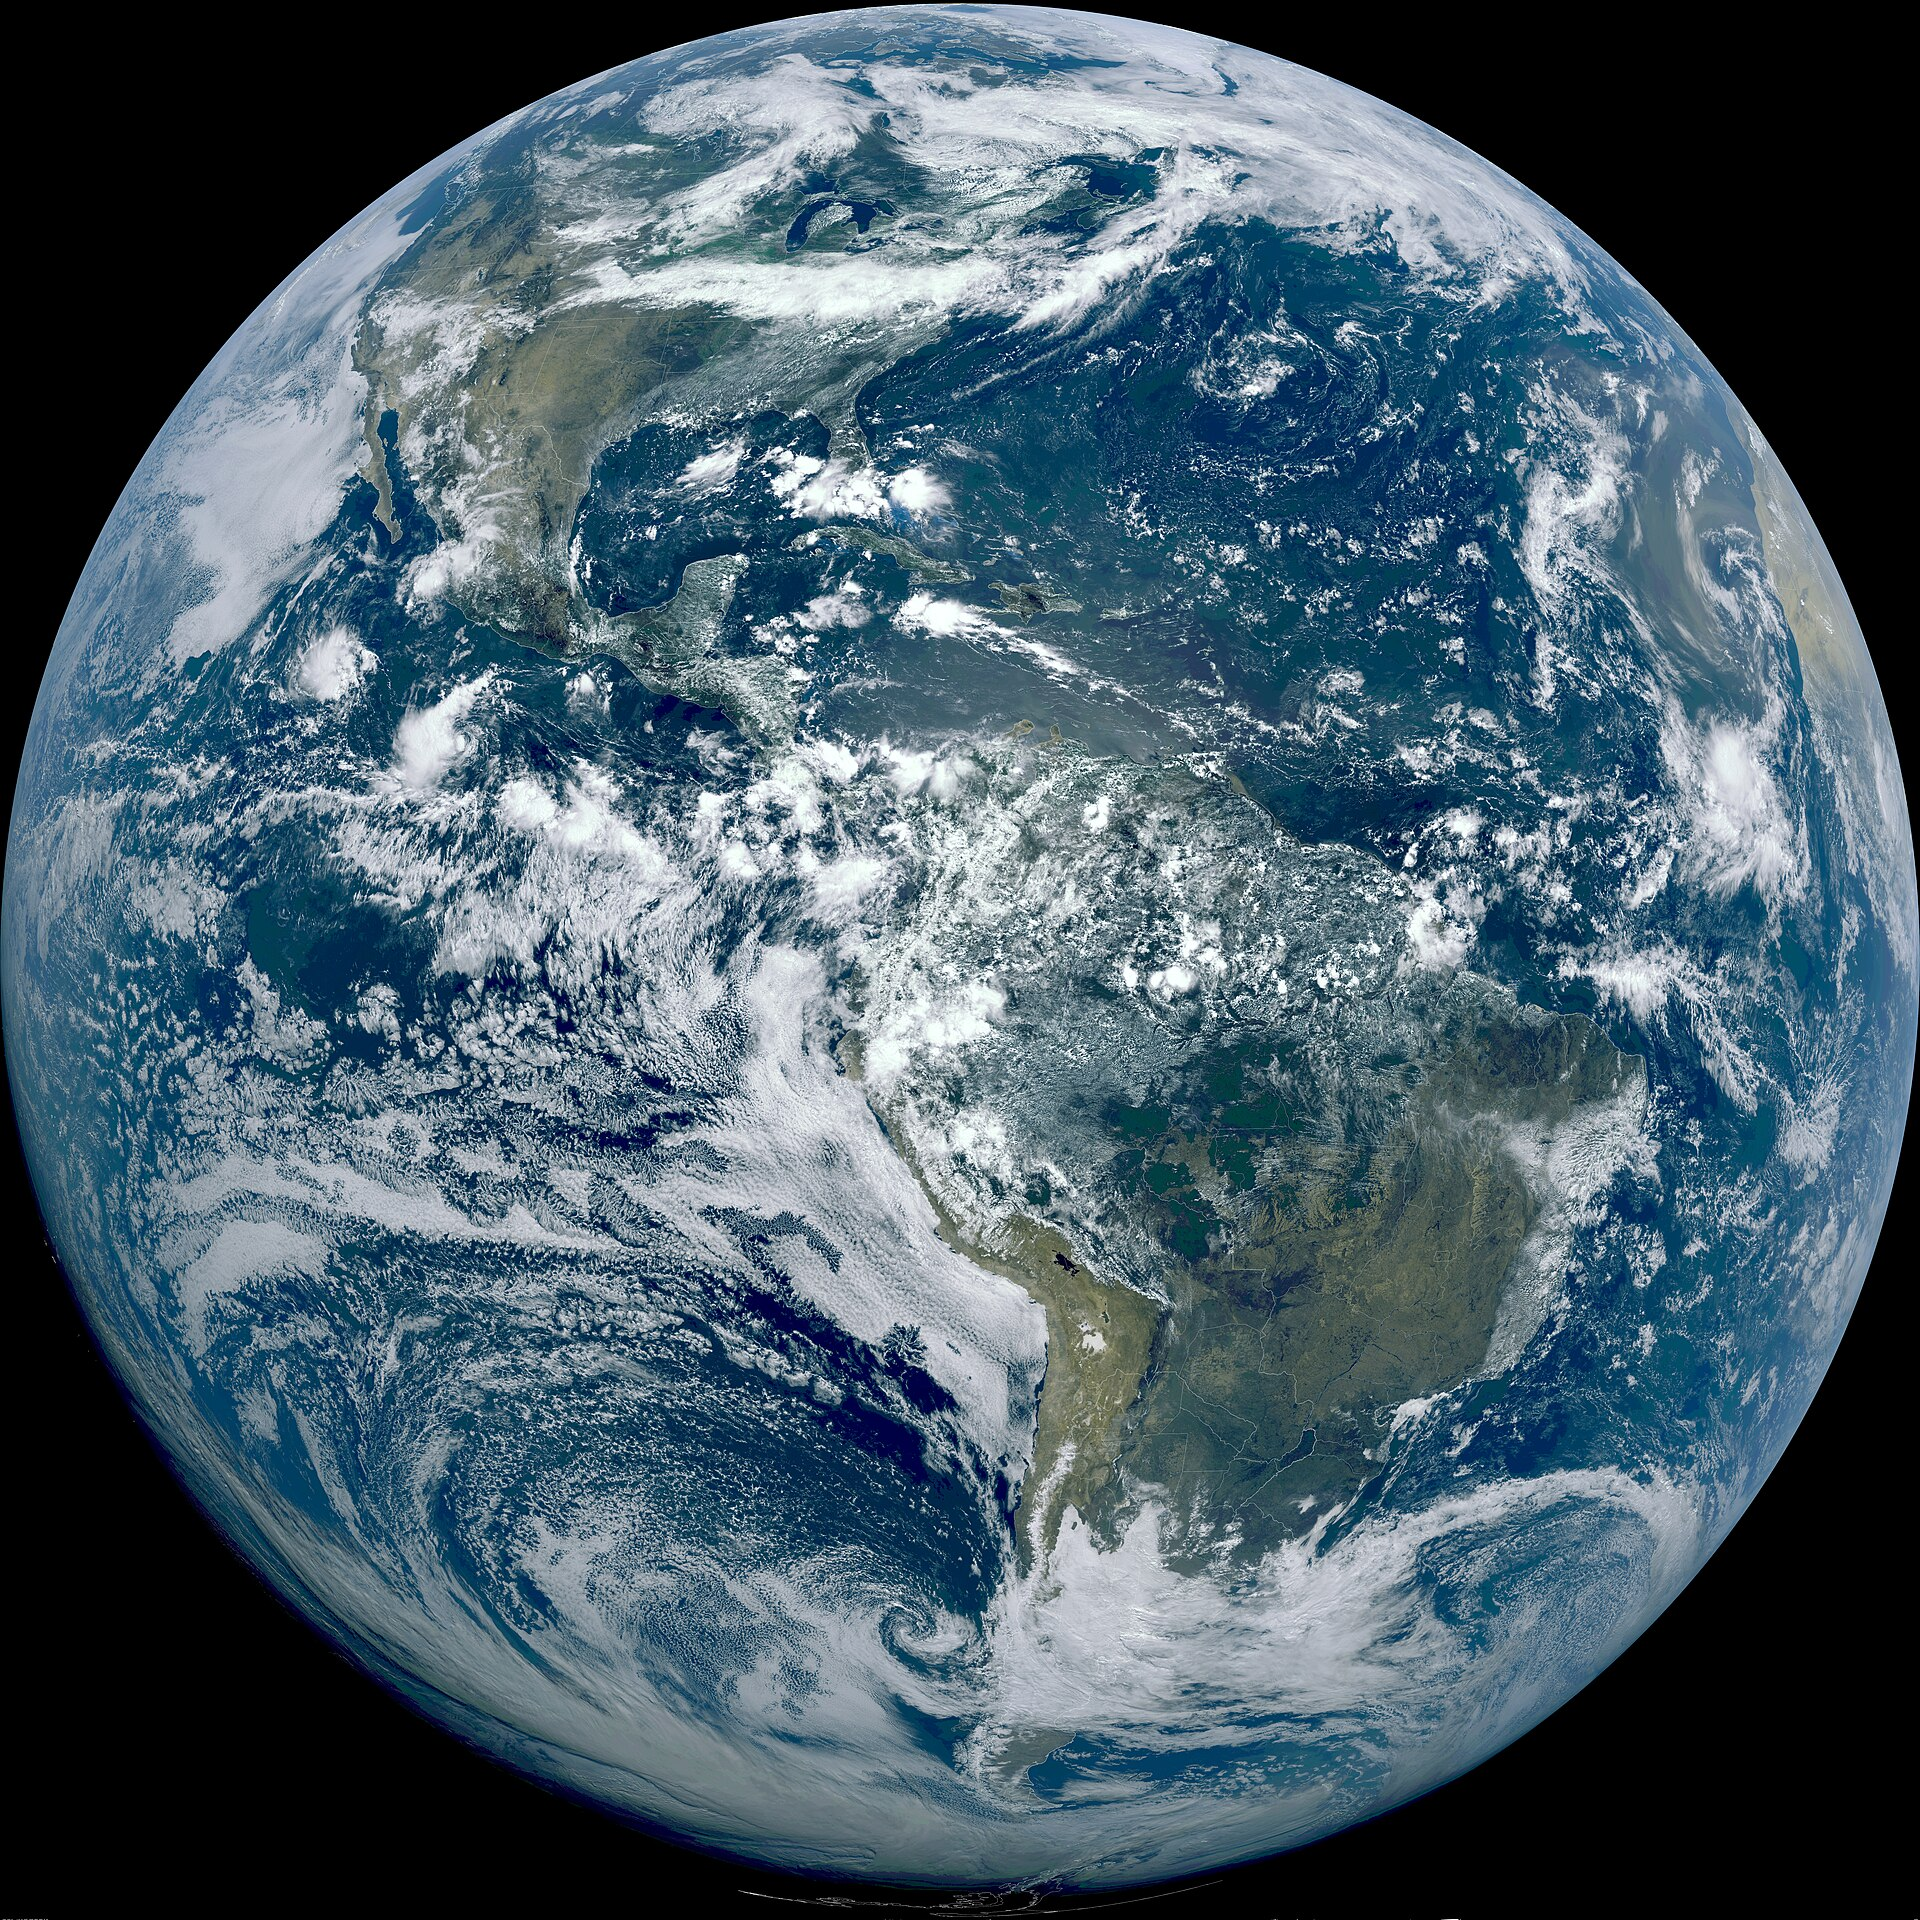
\includegraphics[width=\linewidth]{images/book1/g8-goes-full-disk.jpg}
\end{minipage}\hfill
\begin{minipage}[c]{0.54\linewidth}\raggedright
{\small As Américas vistas pelo satélite meteorológico GOES-16, bem acima
do \omterm{def:g3:continents-and-oceans:equator}{equador}, em 26~de~julho~de~2022. Muitas \omterm{def:g4:clouds-rain-snow:cloud}{nuvens} se formaram sobre os
\omterm{def:g5:weather-and-climate:tropics}{trópicos} e sobre a floresta amazônica, onde o ar quente e úmido sobe;
bem ao sul, no inverno austral, as \omterm{def:g5:natural-hazards:storm}{tempestades} dos \omterm{def:g8:winds-global-circulation:global-winds}{ventos de oeste}
giram sobre o \omterm{def:g2:water-on-earth:ocean}{oceano}. NOAA (domínio público, via Wikimedia Commons).}
\end{minipage}
% ledger: commons:goes16, nos:doldrums
\label{fig:g8:winds-global-circulation:goes}
\end{omfigure}

\begin{example}[Quatro cidades, quatro faixas]\label{ex:g8:winds-global-circulation:four-towns}
As quatro cidades dos \omterm{def:g5:weather-and-climate:climate-chart}{climogramas} do \cref{ch:g5:weather-and-climate}
ficam todas no \omterm{def:g3:continents-and-oceans:equator}{hemisfério norte}, em \omterm{def:g6:latitude-longitude:latitude}{latitudes} muito diferentes. A sua
\omterm{def:g4:clouds-rain-snow:precipitation}{chuva} e a sua \omterm{def:g4:clouds-rain-snow:precipitation}{neve} de um ano seguem as faixas da \omterm{def:g8:winds-global-circulation:circulation}{circulação geral}
(gráfico abaixo). Hilo, a \ang{20}\,N, fica numa ilha na faixa dos
\omterm{def:g8:winds-global-circulation:global-winds}{alísios}, no meio do \omterm{def:g2:water-on-earth:ocean}{oceano}, onde os \omterm{def:g8:winds-global-circulation:global-winds}{alísios} recolhem vapor de água: cerca
de \qty{3000}{mm} caem ali num ano. Phoenix, a \ang{33}\,N, fica perto de
\ang{30}, embaixo do ar que desce: menos de \qty{200}{mm}. Seattle, a
\ang{47}\,N, fica nos \omterm{def:g8:winds-global-circulation:global-winds}{ventos de oeste}, cujas \omterm{def:g5:natural-hazards:storm}{tempestades} trazem cerca de
\qty{1000}{mm} por ano, a maior parte do outono à primavera. Utqiaġvik, a
\ang{71}\,N, fica embaixo do ar frio que desce perto do \omterm{def:g3:continents-and-oceans:poles}{polo}: menos de
\qty{150}{mm}, um \omterm{def:g5:weather-and-climate:desert}{deserto} frio.
% ledger: data:b1-noaa-normals (totals from figdata/grade-5/climate_charts.py, re-read in figdata/grade-8/rain_by_belt.py), mo:three-cells, nos:doldrums
\end{example}

\begin{omfigure}
\begin{tikzpicture}
\begin{axis}[xbar, width=0.82\linewidth, height=6.4cm, bar width=9pt,
  xmin=0, xmax=3600, ymin=0, ymax=90, ytick={0,30,60,90},
  yticklabels={$0^\circ$, $30^\circ$\,N, $60^\circ$\,N, $90^\circ$\,N},
  xlabel={chuva e neve num ano (mm)}, ylabel={latitude},
  axis x line=bottom, axis y line=left, axis line style={-},
  tick label style={font=\scriptsize}, label style={font=\small},
  xtick={0,1000,2000,3000}, scaled x ticks=false, clip=false,
  point meta=explicit symbolic, nodes near coords,
  nodes near coords style={font=\scriptsize, anchor=west}]
  \draw[black!35, dashed] (axis cs:0,30) -- (axis cs:3600,30);
  \draw[black!35, dashed] (axis cs:0,60) -- (axis cs:3600,60);
  \node[font=\scriptsize, black!60, anchor=south east] at (axis cs:3600,1) {ar que sobe: chuva};
  \node[font=\scriptsize, black!60, anchor=south east] at (axis cs:3600,30) {ar que desce: árido};
  \node[font=\scriptsize, black!60, anchor=south east] at (axis cs:3600,60) {ar que sobe: chuva};
  \node[font=\scriptsize, black!60, anchor=north east] at (axis cs:3600,90) {ar que desce: árido};
  \addplot[fill=blue!35, draw=blue!60!black] table[x=total_mm, y=lat, meta=name] {figdata/out/grade-8-rain_by_belt-stations.dat};
\end{axis}
\end{tikzpicture}

{\small \omterm{def:g4:clouds-rain-snow:precipitation}{Chuva} e \omterm{def:g4:clouds-rain-snow:precipitation}{neve} de um ano (médias de 1991--2020) das quatro cidades
dos \omterm{def:g5:weather-and-climate:climate-chart}{climogramas}, colocadas nas suas \omterm{def:g6:latitude-longitude:latitude}{latitudes}. As cidades úmidas ficam
onde o ar sobe, perto do \omterm{def:g3:continents-and-oceans:equator}{equador} e perto de \ang{60}; as áridas, onde ele
desce, perto de \ang{30} e perto do \omterm{def:g3:continents-and-oceans:poles}{polo}. Normais climatológicas da NOAA.}
% ledger: data:b1-noaa-normals, mo:three-cells (figdata/grade-8/rain_by_belt.py)
\end{omfigure}

Quatro cidades são só quatro pontos: as \omterm{def:g1:landscapes-around-us:landform}{montanhas}, os \omterm{def:g1:landscapes-around-us:water}{litorais} e os \omterm{def:g2:water-on-earth:ocean}{mares}
frios ou quentes também mudam a quantidade de \omterm{def:g4:clouds-rain-snow:precipitation}{chuva} que um lugar recebe.
As faixas dão o desenho geral do \omterm{def:g2:drawing-to-map:map}{mapa} dos \omterm{def:g5:weather-and-climate:climate}{climas}, e não a \omterm{def:g4:clouds-rain-snow:precipitation}{chuva} de cada
cidade.

\section{Exercícios}

\begin{exercise}[$\star$]\label{exo:g8:winds-global-circulation:1}
Dê o nome do vento global que sopra com mais frequência: (a) a \ang{15}
norte; (b) a \ang{45} sul; (c) a \ang{75} norte; (d) a \ang{20} sul. Dê
a sua direção a cada vez.
\end{exercise}

\begin{exercise}[$\star$]\label{exo:g8:winds-global-circulation:2}
Complete cada frase. (a) O ar quente \dots\ e o ar frio \dots. (b) Embaixo
do ar que sobe, a pressão no chão é \dots. (c) No chão, o vento sopra da
pressão \dots\ para a pressão \dots. (d) No \omterm{def:g3:continents-and-oceans:equator}{hemisfério norte}, a rotação
da Terra desvia o ar em movimento para a \dots.
\end{exercise}

\begin{exercise}[$\star$]\label{exo:g8:winds-global-circulation:3}
Verdadeiro ou falso? Corrija as frases falsas. (a) Uma \omterm{def:g8:winds-global-circulation:breezes}{brisa marítima}
sopra da terra para o \omterm{def:g2:water-on-earth:ocean}{mar}. (b) De dia, a terra esquenta mais depressa que
o \omterm{def:g2:water-on-earth:ocean}{mar}. (c) Os \omterm{def:g8:winds-global-circulation:global-winds}{alísios} sopram do oeste. (d) Muitos grandes \omterm{def:g5:weather-and-climate:desert}{desertos} ficam
perto de \ang{30} de \omterm{def:g6:latitude-longitude:latitude}{latitude}.
\end{exercise}

\begin{exercise}[$\star$]\label{exo:g8:winds-global-circulation:4}
Desenhe um \omterm{def:g1:landscapes-around-us:water}{litoral} com o \omterm{def:g2:water-on-earth:ocean}{mar} à esquerda e a terra à direita. Acrescente o
Sol, e depois desenhe com setas o circuito de ar da \omterm{def:g8:winds-global-circulation:breezes}{brisa marítima}. Marque
H e L onde a pressão no chão é alta e baixa.
\end{exercise}

\begin{exercise}[$\star\star$]\label{exo:g8:winds-global-circulation:5}
Use a tabela dos feixes deste capítulo. (a) A \ang{45}, quanto chão a
mais um feixe cobre em comparação com o \omterm{def:g3:continents-and-oceans:equator}{equador}? (b) Que porcentagem da
energia do \omterm{def:g3:continents-and-oceans:equator}{equador} cada metro quadrado recebe a \ang{60}? (c) E a
\ang{75}? (d) Explique numa frase por que os \omterm{def:g3:continents-and-oceans:poles}{polos} são frios.
\end{exercise}

\begin{exercise}[$\star\star$]\label{exo:g8:winds-global-circulation:6}
Um barco navega bem para o sul através do \omterm{def:g3:continents-and-oceans:equator}{hemisfério norte} e depois do
\omterm{def:g3:continents-and-oceans:equator}{hemisfério sul}. (a) Que ventos ele encontra, em ordem, de \ang{70} N até
\ang{70} S? (b) Onde ele provavelmente vai encontrar ar calmo e pancadas de
\omterm{def:g4:clouds-rain-snow:precipitation}{chuva} frequentes? (c) Onde os ventos são fracos e a \omterm{def:g4:clouds-rain-snow:precipitation}{chuva} é rara?
\end{exercise}

\begin{exercise}[$\star\star$]\label{exo:g8:winds-global-circulation:7}
Numa praia, faz \qty{31}{\degreeCelsius} sobre a \omterm{def:g3:stones-pebbles-sand:sand}{areia} às 15~h e
\qty{22}{\degreeCelsius} sobre o \omterm{def:g2:water-on-earth:ocean}{mar}. Às 3~h, faz
\qty{17}{\degreeCelsius} sobre a terra e \qty{21}{\degreeCelsius} sobre o
\omterm{def:g2:water-on-earth:ocean}{mar}. (a) O que está mais quente às 15~h? Para que lado sopra o vento?
(b) E às 3~h? (c) Quantos graus a temperatura da terra muda entre os dois
horários? E a do \omterm{def:g2:water-on-earth:ocean}{mar}? (d) Explique a diferença.
\end{exercise}

\begin{exercise}[$\star\star$]\label{exo:g8:winds-global-circulation:8}
O ar corre da faixa de alta pressão perto de \ang{30} N em direção ao
\omterm{def:g3:continents-and-oceans:equator}{equador}. (a) Sem a rotação da Terra, de que direção ele sopraria? (b) Para
que lado a rotação o desvia nesse \omterm{def:g3:continents-and-oceans:equator}{hemisfério}? (c) De que direção ele sopra
então? (d) Responda às mesmas três perguntas para o ar que corre em
direção ao \omterm{def:g3:continents-and-oceans:equator}{equador} a partir de \ang{30} S.
\end{exercise}

\begin{exercise}[$\star\star$]\label{exo:g8:winds-global-circulation:9}
Explique, passo a passo, por que chove tanto perto do \omterm{def:g3:continents-and-oceans:equator}{equador}: use as
palavras \emph{aquecido}, \emph{sobe}, \emph{esfria}, \emph{\omterm{def:g4:clouds-rain-snow:cloud}{nuvens}}.
Depois, explique por que há um \omterm{def:g5:weather-and-climate:desert}{deserto} perto de \ang{25} N, no norte da
África: use as palavras \emph{desce}, \emph{alta pressão}, \emph{árido}.
\end{exercise}

\begin{exercise}[$\star\star$]\label{exo:g8:winds-global-circulation:10}
Um veleiro sai de um porto a \ang{40} N, na costa oeste da Europa, para o
Caribe, a \ang{15} N. (a) Que vento ele encontraria a \ang{40} N? Esse
vento ajudaria o navio a navegar para o oeste? (b) Por que o navio deveria
primeiro navegar para o sul? (c) Que vento o leva para o oeste, e entre
que \omterm{def:g6:latitude-longitude:latitude}{latitudes}? (d) Para a viagem de volta à Europa, que vento o navio
deveria procurar, e em que \omterm{def:g6:latitude-longitude:latitude}{latitude}?
\end{exercise}

\begin{exercise}[$\star\star\star$]\label{exo:g8:winds-global-circulation:11}
Na \omterm{def:g6:latitude-longitude:latitude}{latitude} $L$, um feixe de luz do Sol ao meio-dia de um equinócio cobre $1 \div
\cos L$ vezes o chão que ele cobre no \omterm{def:g3:continents-and-oceans:equator}{equador} (numa calculadora,
$\cos 60^\circ = 0.5$). (a) Verifique o valor para \ang{60}. (b) Usando
$\cos 30^\circ \approx 0.866$, verifique o valor para \ang{30}, arredondado
para duas casas decimais. (c) Suponha que um painel solar deitado recebe
\qty{1000}{W} em cada metro quadrado ao meio-dia no \omterm{def:g3:continents-and-oceans:equator}{equador} nesse dia.
Aproximadamente quanto o mesmo painel receberia a \ang{30}? E a \ang{60}?
\end{exercise}

\begin{exercise}[$\star\star\star$]\label{exo:g8:winds-global-circulation:12}
Em cada \omterm{def:g3:continents-and-oceans:equator}{hemisfério}, a \omterm{def:g8:winds-global-circulation:circulation}{circulação geral} tem três células. (a) Desenhe uma
vista de lado do \omterm{def:g3:continents-and-oceans:equator}{hemisfério norte}, com o \omterm{def:g3:continents-and-oceans:equator}{equador} embaixo e o \omterm{def:g3:continents-and-oceans:poles}{polo} em cima,
e as três células como circuitos; mostre onde o ar sobe e onde ele desce.
(b) Marque as faixas de alta e de baixa pressão no chão. (c) Acrescente
os ventos de superfície de cada célula, desviados para a direita.
(d) Use o seu desenho para explicar por que os \omterm{def:g8:winds-global-circulation:global-winds}{ventos de oeste} sopram em
direção ao nordeste.
\end{exercise}

\section{Problema: Navegar com os alísios}

\begin{problem}[{Problema de fim de semana --- um veleiro atravessa o
Atlântico de Cabo Verde a Barbados com o alísio de nordeste; a rota é
medida no mapa, o vento é lido, e calcula-se a duração da
travessia}]
\label{pb:g8:winds-global-circulation:1}
% ledger: data:b1-ne-places, earth:Rmean, nos:trade-winds (figdata/grade-8/trade_route.py; the speed is exercise data)
Um veleiro sai de Praia, nas ilhas de Cabo Verde, para Bridgetown, em
Barbados. O \omterm{def:g2:drawing-to-map:map}{mapa} mostra a rota e o alísio.

\begin{center}
\begin{tikzpicture}
\begin{axis}[ommap, width=12cm, xmin=-75, xmax=-5, ymin=0, ymax=35, axis equal image,
  xtick={-70,-60,-50,-40,-30,-20,-10}, ytick={0,10,20,30},
  tick label style={font=\scriptsize},
  xlabel={longitude (negativa = oeste)}, ylabel={latitude (norte)},
  label style={font=\small}, clip mode=individual]
  \addplot[fill=omLithAlluv, draw=black!60, line width=0.3pt] table {figdata/out/grade-8-trade_route-land.dat};
  \addplot[quiver={u=\thisrow{dlon}, v=\thisrow{dlat}}, -{Stealth[length=1.6mm]}, omThm!80, line width=0.7pt]
    table[x=lon, y=lat] {figdata/out/grade-8-trade_route-trades.dat};
  \addplot[omDef, line width=1.3pt, dashed] table {figdata/out/grade-8-trade_route-route.dat};
  \addplot[only marks, mark=*, mark size=2pt, black] table[x=lon, y=lat] {figdata/out/grade-8-trade_route-ports.dat};
  \node[anchor=north, font=\scriptsize\bfseries, fill=white, inner sep=1pt] at (axis cs:-59.6,12.2) {Bridgetown};
  \node[anchor=south, font=\scriptsize\bfseries, fill=white, inner sep=1pt] at (axis cs:-23.5,15.8) {Praia};
\end{axis}
\end{tikzpicture}
\end{center}

\noindent\textbf{Parte I --- A rota.}\par\nopagebreak
\begin{enumerate}[beginpenalty=10000]
  \item Praia fica a \ang{14.9} N, \ang{23.5} O; Bridgetown, a
        \ang{13.1} N, \ang{59.6} O. Quantos graus de \omterm{def:g6:latitude-longitude:longitude}{longitude} separam as
        duas?
  \item Os dois portos ficam perto de \ang{14} N. Ao longo desse
        \omterm{def:g6:latitude-longitude:latitude}{paralelo}, um grau de \omterm{def:g6:latitude-longitude:longitude}{longitude} mede cerca de \qty{108}{km}. Quantos
        quilômetros tem a travessia, aproximadamente? Arredonde para a
        centena mais próxima.
  \item Medida exatamente sobre a Terra redonda, a rota mais curta tem
        \qty{3896}{km}. A resposta da questão 2 é uma boa estimativa?
  \item Os portos ficam na faixa dos \omterm{def:g8:winds-global-circulation:global-winds}{alísios}? Explique.
\end{enumerate}

\noindent\textbf{Parte II --- O vento.}\par\nopagebreak
\begin{enumerate}[resume, beginpenalty=10000]
  \item De que direção sopra o alísio aqui?
  \item O navio navega para o oeste. O vento o empurra para a frente, para
        trás ou para o lado? Explique com o \omterm{def:g2:drawing-to-map:map}{mapa}.
  \item Por que o alísio sopra na mesma direção quase todos os dias da
        travessia?
  \item Na volta para a Europa, por que o capitão não deveria tentar
        navegar para o leste ao longo de \ang{14} N?
\end{enumerate}

\noindent\textbf{Parte III --- A travessia.}\par\nopagebreak
\begin{enumerate}[resume, beginpenalty=10000]
  \item Suponha que o navio faz em média \qty{7}{km} por hora. Quantos
        quilômetros ele percorre num dia de 24 horas?
  \item Se o vento parasse durante 3 dias no caminho, quantos quilômetros
        de progresso o navio perderia?
  \item Com um alísio constante, de quantos dias o navio precisa para
        \qty{3896}{km}? Arredonde para uma casa decimal.
  \item Arredondando para o dia inteiro mais próximo, quanto tempo dura a
        travessia? É mais ou menos que um mês?
\end{enumerate}
\end{problem}
